\documentclass[11pt]{article}

\usepackage[a4paper,margin=2.5cm]{geometry}
\usepackage{amsmath,amssymb,amsfonts}
\usepackage{graphicx}
\usepackage{booktabs}
\usepackage{float}
\usepackage[hidelinks]{hyperref}
\usepackage{bookmark}
\usepackage{caption}
\usepackage{subcaption}


\title{Nesterov's smooth minimization of non-smooth functions}
\author{Michał Szewczak, Sebastian Trojan}
\date{}

\begin{document}

\maketitle

\begin{abstract}

This report studies Nesterov's smoothing technique for structured non-smooth
convex optimization problems. The method applies to objectives whose
non-smooth part can be written as a maximization over an auxiliary variable.
This maximization is regularized by a strongly convex prox-function, producing
a smooth approximation with an explicit error bound. The resulting smooth
problem is solved by an accelerated first-order method, and convergence is
measured by a primal-dual gap certificate.

The implementation is tested on matrix games, the continuous location problem,
and two absolute-value objectives: the maximum of absolute values and the sum
of absolute values. The experiments reproduce the qualitative behavior of
Nesterov's matrix game example, compare several problem classes, examine the
empirical dependence of the iteration count on the accuracy parameter
\(\varepsilon\), and test a continuation strategy in which the smoothing
parameter is decreased during optimization.

\end{abstract}

\tableofcontents
\newpage


\section{Introduction}

Many convex optimization problems are non-smooth because their objectives
contain maxima, norms, or absolute values. Such functions are still convex, but
standard gradient methods cannot be applied directly, and classical subgradient
methods usually have a slow worst-case convergence rate. Nesterov's smoothing
method addresses this difficulty for a special but important class of
non-smooth problems: those whose non-smooth term has an explicit maximization
structure.

The central idea is to replace the auxiliary maximization by a regularized
maximization. The regularization is controlled by a smoothing parameter
\(\mu\). A larger value of \(\mu\) gives a smoother and easier problem, while a
smaller value gives a more accurate approximation of the original non-smooth
objective. This creates a trade-off between approximation accuracy and the
conditioning of the smoothed problem.

The aim of this report is to implement and experimentally study this smoothing
framework. First, the theoretical construction from Nesterov's paper is
summarized: the structured problem class, the smooth approximation, the
accelerated method, the primal-dual gap certificate, and the resulting
\(O(1/\varepsilon)\) complexity bound. Next, the problem classes used in the
experiments are introduced. Finally, computational experiments are presented for
matrix games, the continuous location problem, the maximum of absolute values
problem, and the sum of absolute values problem.

The experiments focus on certified convergence. Instead of reporting only
objective values, the stopping criterion is the primal-dual gap, which gives an
explicit certificate that the returned solution is \(\varepsilon\)-optimal. The
experiments also compare the theoretical iteration prediction with observed
iteration counts and test whether a practical continuation strategy for the
smoothing parameter can improve performance.

\section{Theoretical Background}

This section describes the theoretical framework used in the implementation.
The method applies to structured non-smooth convex problems whose non-smooth
part is written as a maximization over an auxiliary variable. Nesterov's
smoothing technique regularizes this maximization with a strongly convex
prox-function. The result is a differentiable approximation with a controlled
approximation error. The smoothed problem is then minimized by an accelerated
first-order method, and the quality of the computed solution is certified by a
primal-dual gap.

\subsection{Problem class}

Nesterov's smoothing technique \cite{nesterov2005smooth} applies to convex
problems of the form
\[
    f^*=\min_{x\in Q_1} f(x),
\]
where \(Q_1\) is a closed convex set. The important assumption is that the
objective has the structured form
\[
    f(x)
    =
    \hat f(x)
    +
    \max_{u\in Q_2}
    \left\{
        \langle Ax,u\rangle-\hat\phi(u)
    \right\}.
\]
Here \(Q_2\) is another closed convex set, \(A\) is a linear operator,
\(\hat f\) is a smooth convex function, and \(\hat\phi\) is a convex function on
\(Q_2\). The non-smoothness comes from the maximization over the auxiliary
variable \(u\). In the examples considered in this report, \(\hat f=0\), so the
objective is generated entirely by the max-term.

The variable \(x\) is the primal variable. The variable \(u\) is the auxiliary,
or dual, variable. For a fixed \(x\), it identifies the active part of the
maximum and is later used to construct the dual certificate.

\subsection{Prox-functions and smoothing}

The method uses prox-functions on the primal and auxiliary feasible sets. Let
\(d_1\) be a prox-function on \(Q_1\), strongly convex with parameter
\(\sigma_1>0\), and let \(d_2\) be a prox-function on \(Q_2\), strongly convex
with parameter \(\sigma_2>0\). As in the paper, the prox-functions are assumed
to be normalized so that their minimum values on the corresponding sets are
zero. Define
\[
    D_1=\max_{x\in Q_1}d_1(x),
    \qquad
    D_2=\max_{u\in Q_2}d_2(u).
\]

For a smoothing parameter \(\mu>0\), the max-term is replaced by
\[
    f_\mu(x)
    =
    \max_{u\in Q_2}
    \left\{
        \langle Ax,u\rangle-\hat\phi(u)-\mu d_2(u)
    \right\}.
\]
The smooth approximation of the full objective is therefore
\[
    \bar f_\mu(x)=\hat f(x)+f_\mu(x).
\]
The additional term \(-\mu d_2(u)\) makes the inner maximization strongly
concave in the dual variable and gives a differentiable approximation.

The approximation error is uniformly bounded:
\[
    \bar f_\mu(x)\le f(x)\le \bar f_\mu(x)+\mu D_2.
\]
Thus \(\mu D_2\) is an upper bound on the smoothing error. Smaller \(\mu\) gives
a more accurate approximation, but it also makes the smoothed function less
smooth.

\subsection{Gradient of the smoothed objective}

For each \(x\), define the smoothed dual response
\[
    u_\mu(x)
    =
    \arg\max_{u\in Q_2}
    \left\{
        \langle Ax,u\rangle-\hat\phi(u)-\mu d_2(u)
    \right\}.
\]
Nesterov shows that the smoothed max-term is differentiable and
\[
    \nabla f_\mu(x)=A^*u_\mu(x).
\]
Consequently,
\[
    \nabla \bar f_\mu(x)
    =
    \nabla\hat f(x)+A^*u_\mu(x).
\]
If \(M\) is the Lipschitz constant of \(\nabla\hat f\), then the gradient of
\(\bar f_\mu\) is Lipschitz continuous with constant
\[
    L_\mu
    =
    M+\frac{\|A\|_{1,2}^2}{\mu\sigma_2}.
\]
This formula is central to the method: decreasing \(\mu\) improves the
approximation error, but increases \(L_\mu\), so the smooth problem becomes
harder for a first-order method.

\subsection{Accelerated minimization of the smoothed problem}

For a the standard method, the algorithm minimizes
\[
    \min_{x\in Q_1}\bar f_\mu(x).
\]
The accelerated scheme used in the paper maintains three sequences
\(x_k,y_k,z_k\). At iteration \(k\), it computes
\[
    g_k=\nabla\bar f_\mu(x_k).
\]
The local point is
\[
    y_k=T_{Q_1}(x_k),
\]
where
\[
    T_{Q_1}(x_k)
    =
    \arg\min_{y\in Q_1}
    \left\{
        \langle g_k,y-x_k\rangle
        +
        \frac{L}{2}\|y-x_k\|^2
    \right\}.
\]
The method also forms an aggregate point from all previous gradients. With
\[
    \alpha_k=\frac{k+1}{2},
    \qquad
    G_k=\sum_{i=0}^k\alpha_i g_i,
\]
define
\[
    z_k
    =
    \arg\min_{x\in Q_1}
    \left\{
        \frac{L}{\sigma_1}d_1(x)+\langle G_k,x\rangle
    \right\}.
\]
The next point is the convex combination
\[
    x_{k+1}
    =
    \frac{2}{k+3}z_k
    +
    \frac{k+1}{k+3}y_k.
\]
This is the accelerated part of the method. In the implementation, the formulas
above are specialized to the geometry of each problem class.

\subsection{Dual averaging and stopping criterion}

At iteration \(k\), the method computes the smoothed dual response
\[
    u_k = u_\mu(x_k).
\]
The final dual candidate is formed as a weighted average of these responses:
\[
    \hat u =
    \frac{\sum_{k=0}^{N}\alpha_k u_k}
         {\sum_{k=0}^{N}\alpha_k},
    \qquad
    \alpha_k=\frac{k+1}{2}.
\]
Equivalently,
\[
    \hat u =
    \sum_{k=0}^{N}
    \frac{2(k+1)}{(N+1)(N+2)}u_k .
\]
Since \(Q_2\) is convex and each \(u_k\in Q_2\), the averaged point also
satisfies \(\hat u\in Q_2\).

After \(N\) iterations, the final primal point is taken to be the last
\(y\)-iterate,
\[
    \hat x = y_N .
\]
The corresponding dual value is defined by
\[
    \phi(u)
    =
    \min_{x\in Q_1}
    \left\{
        \hat f(x)+\langle Ax,u\rangle
    \right\}
    -\hat\phi(u).
\]
By weak duality,
\[
    \phi(\hat u)\le f^*\le f(\hat x).
\]
Therefore,
\[
    f(\hat x)-\phi(\hat u)
\]
is a primal-dual gap. In the implementation, this quantity is used as the
stopping criterion. The algorithm stops when
\[
    f(\hat x)-\phi(\hat u)\le \varepsilon.
\]
This gives a certificate that the computed point is \(\varepsilon\)-optimal.

\subsection{Complexity bound}

Nesterov's analysis chooses the smoothing parameter as a function of the planned
number of iterations. For a fixed number \(N\), the smoothing parameter is chosen
as
\[
    \mu(N)
    =
    \frac{2\|A\|_{1,2}}{N+1}
    \sqrt{
        \frac{D_1}{\sigma_1\sigma_2D_2}
    }.
\]
With this choice, the method gives the primal-dual estimate
\[
    0
    \le
    f(\hat x)-\phi(\hat u)
    \le
    \frac{4\|A\|_{1,2}}{N+1}
    \sqrt{
        \frac{D_1D_2}{\sigma_1\sigma_2}
    }
    +
    \frac{4MD_1}{\sigma_1(N+1)^2}.
\]
Here \(M\) is the Lipschitz constant of \(\nabla\hat f\). In the examples
implemented in this project, \(\hat f=0\), so \(M=0\). The bound then becomes
\[
    f(\hat x)-\phi(\hat u)
    \le
    \frac{4\|A\|_{1,2}}{N+1}
    \sqrt{
        \frac{D_1D_2}{\sigma_1\sigma_2}
    }.
\]

If the required accuracy is fixed in advance, this estimate can be rewritten in
terms of \(\varepsilon\). To guarantee
\[
    f(\hat x)-\phi(\hat u)\le\varepsilon,
\]
it is sufficient to take
\[
    N+1
    \ge
    \frac{4\|A\|_{1,2}}{\varepsilon}
    \sqrt{
        \frac{D_1D_2}{\sigma_1\sigma_2}
    }.
\]
Substituting this value of \(N+1\) into \(\mu(N)\) gives the equivalent
accuracy-based choice
\[
    \mu
    =
    \frac{\varepsilon}{2D_2}.
\]
Thus the smoothing error satisfies
\[
    \mu D_2=\frac{\varepsilon}{2}.
\]

For this choice of \(\mu\), the Lipschitz constant of the smoothed objective is
\[
    L_\mu
    =
    M+
    \frac{\|A\|_{1,2}^2}{\mu\sigma_2}
    =
    M+
    \frac{2D_2}{\sigma_2}
    \frac{\|A\|_{1,2}^2}{\varepsilon}.
\]
When \(M=0\), this simplifies to
\[
    L_\mu
    =
    \frac{2D_2}{\sigma_2}
    \frac{\|A\|_{1,2}^2}{\varepsilon}.
\]

The resulting theoretical iteration complexity is therefore
\[
    N=O\left(\frac{1}{\varepsilon}\right).
\]
This is the predicted iteration bound used later in the computational
experiments.



\section{Problem Classes}

This section presents the problem classes used in the experiments. All of them
are based on application examples discussed by Nesterov. The goal is to show how
each problem can be written in the structured form
\[
    \min_{x\in Q_1}
    \left\{
        \hat f(x)
        +
        \max_{u\in Q_2}
        \left(
            \langle Ax,u\rangle-\hat\phi(u)
        \right)
    \right\}.
\]
In all examples considered here, \(\hat f(x)=0\). Thus, the essential step is
to express the non-smooth objective as a maximization over an auxiliary
variable.

\subsection{Matrix games}

The matrix game problem is
\[
    \min_{x\in\Delta_n}
    \max_{u\in\Delta_m}
    u^\top Ax,
\]
where \(A\in\mathbb{R}^{m\times n}\), and \(\Delta_n,\Delta_m\) are probability
simplexes. This problem can be interpreted as a two-player zero-sum game. The
vector \(x\) is the mixed strategy of the minimizing player, while \(u\) is the
mixed strategy of the maximizing player.

The problem already has the required max-structure, because
\[
    u^\top Ax=\langle Ax,u\rangle.
\]
Thus,
\[
    Q_1=\Delta_n,
    \qquad
    Q_2=\Delta_m,
    \qquad
    \hat\phi(u)=0.
\]
The final form is
\[
    \boxed{
    \min_{x\in\Delta_n}
    \max_{u\in\Delta_m}
    \langle Ax,u\rangle .
    }
\]
Equivalently,
\[
    \max_{u\in\Delta_m}u^\top Ax
    =
    \max_{1\le j\le m}(Ax)_j,
\]
so the objective is the maximum of finitely many linear functions.

\subsection{Continuous location problem}

The continuous location problem is
\[
    \min_{\|x\|_2\le r}
    \sum_{j=1}^{p}w_j\|x-c_j\|_2.
\]
Here \(x\) is the location of a facility, \(c_j\) are fixed city or customer
locations, and \(w_j>0\) are weights. The objective is the total weighted
distance from the facility to the given points.

The Euclidean norm has the representation
\[
    \|x-c_j\|_2
    =
    \max_{\|u_j\|_2\le 1}
    \langle x-c_j,u_j\rangle.
\]
Applying this to each distance term gives
\[
    \sum_{j=1}^{p}w_j\|x-c_j\|_2
    =
    \max_{\|u_j\|_2\le 1}
    \left\{
        \sum_{j=1}^{p}w_j\langle x,u_j\rangle
        -
        \sum_{j=1}^{p}w_j\langle c_j,u_j\rangle
    \right\}.
\]

The primal feasible set is
\[
    Q_1=\{x:\|x\|_2\le r\}.
\]
The auxiliary variable is \(U=(u_1,\ldots,u_p)\), with
\[
    Q_2=
    \left\{
        U=(u_1,\ldots,u_p):
        \|u_j\|_2\le 1,\ j=1,\ldots,p
    \right\}.
\]
With the operator
\[
    \mathcal A x=(w_1x,\ldots,w_px),
\]
we have
\[
    \langle \mathcal A x,U\rangle
    =
    \sum_{j=1}^{p}w_j\langle x,u_j\rangle.
\]
Therefore,
\[
    \hat\phi(U)=
    \sum_{j=1}^{p}w_j\langle c_j,u_j\rangle.
\]
The final form is
\[
    \boxed{
    \min_{\|x\|_2\le r}
    \max_{\|u_j\|_2\le 1}
    \left\{
        \sum_{j=1}^{p}w_j\langle x,u_j\rangle
        -
        \sum_{j=1}^{p}w_j\langle c_j,u_j\rangle
    \right\}.
    }
\]


\subsection{Maximum of absolute values problem}

The maximum of absolute values problem is
\[
    \min_{\|x\|_2\le r}
    \max_{1\le j\le m}|a_j^\top x-b_j|.
\]
This problem minimizes the worst absolute residual among the affine expressions
\(a_j^\top x-b_j\).

Let
\[
    A=
    \begin{bmatrix}
        a_1^\top\\
        \vdots\\
        a_m^\top
    \end{bmatrix},
    \qquad
    b=
    \begin{bmatrix}
        b_1\\
        \vdots\\
        b_m
    \end{bmatrix}.
\]
Using
\[
    |a_j^\top x-b_j|
    =
    \max\{a_j^\top x-b_j,\,-a_j^\top x+b_j\},
\]
define
\[
    \widetilde A=
    \begin{bmatrix}
        A\\
        -A
    \end{bmatrix},
    \qquad
    \widetilde b=
    \begin{bmatrix}
        -b\\
        b
    \end{bmatrix}.
\]
Then
\[
    \max_{1\le j\le m}|a_j^\top x-b_j|
    =
    \max_{1\le \ell\le 2m}
    (\widetilde A x+\widetilde b)_\ell.
\]
A maximum of coordinates can be written as a maximization over the simplex:
\[
    \max_{1\le \ell\le 2m}
    (\widetilde A x+\widetilde b)_\ell
    =
    \max_{u\in\Delta_{2m}}
    u^\top(\widetilde A x+\widetilde b).
\]

Thus,
\[
    Q_1=\{x:\|x\|_2\le r\},
    \qquad
    Q_2=\Delta_{2m},
    \qquad
    \hat f(x)=0,
    \qquad
    \hat\phi(u)=-\widetilde b^\top u.
\]
The final form is
\[
    \boxed{
    \min_{\|x\|_2\le r}
    \max_{u\in\Delta_{2m}}
    \left\{
        \langle \widetilde A x,u\rangle
        +
        \widetilde b^\top u
    \right\}.
    }
\]

\subsection{Sum of absolute values problem}

The sum of absolute values problem is
\[
    \min_{\|x\|_2\le r}
    \sum_{j=1}^{m}|a_j^\top x-b_j|.
\]
This problem minimizes the total absolute residual over all affine expressions
\(a_j^\top x-b_j\).

The identity
\[
    |t|=\max_{|u|\le 1}ut
\]
gives
\[
    |a_j^\top x-b_j|
    =
    \max_{|u_j|\le 1}
    u_j(a_j^\top x-b_j).
\]
Since the variables \(u_j\) are chosen independently,
\[
    \sum_{j=1}^{m}|a_j^\top x-b_j|
    =
    \max_{\|u\|_\infty\le 1}
    \sum_{j=1}^{m}u_j(a_j^\top x-b_j).
\]
Expanding the expression gives
\[
    \sum_{j=1}^{m}u_j(a_j^\top x-b_j)
    =
    \langle Ax,u\rangle-b^\top u.
\]

Thus,
\[
    Q_1=\{x:\|x\|_2\le r\},
    \qquad
    Q_2=\{u:\|u\|_\infty\le 1\}=[-1,1]^m,
    \qquad
    \hat f(x)=0,
    \qquad
    \hat\phi(u)=b^\top u.
\]
The final form is
\[
    \boxed{
    \min_{\|x\|_2\le r}
    \max_{\|u\|_\infty\le 1}
    \left\{
        \langle Ax,u\rangle-b^\top u
    \right\}.
    }
\]




\section{Changing the Smoothing Parameter}
\label{sec:changing-mu}

The smoothing parameter controls the trade-off between accuracy and smoothness.
For a prescribed accuracy \(\varepsilon\), the implementation of Nesterov's
smoothing method uses
\[
    \mu_\varepsilon=\frac{\varepsilon}{2D_2}.
\]
This choice makes the smoothing error bounded by
\[
    \mu_\varepsilon D_2=\frac{\varepsilon}{2}.
\]
The remaining part of the error is then controlled by the accelerated
minimization of the smoothed objective.

When high accuracy is required, \(\mu_\varepsilon\) becomes small. This gives a
sharper approximation of the original objective, but it also increases the
Lipschitz constant
\[
    L_\mu
    =
    M+
    \frac{\|A\|_{1,2}^2}{\mu\sigma_2}.
\]
Thus the smoothed problem can become harder to minimize.

This motivates a continuation strategy. The final accuracy requirement is not
changed, but the method reaches the final smoothing parameter gradually. It
starts from a larger value
\[
    \mu_0=c\mu_\varepsilon,\qquad c>1,
\]
and decreases the smoothing parameter geometrically,
\[
    \mu_{t+1}=\rho\mu_t,\qquad 0<\rho<1,
\]
until \(\mu_\varepsilon\) is reached. At each stage, the accelerated method is
applied to the smoothed problem with the current value \(\mu_t\). The transition
to the next stage is made after the current primal-dual gap reaches a prescribed
intermediate tolerance, for example
\[
    f(\hat x)-\phi(\hat u)
    \le
    c_{\mathrm{stage}}\mu_tD_2,
\]
where \(c_{\mathrm{stage}}>0\) determines how accurately the intermediate stage
is solved. At the last stage, the usual final condition is imposed:
\[
    f(\hat x)-\phi(\hat u)\le \varepsilon.
\]

The continuation strategy is a practical modification of the standard smoothing
method. It is tested in this report to see whether progress made on smoother
intermediate problems can reduce the total computational effort. The concrete
values of \(c\), \(\rho\), and \(c_{\mathrm{stage}}\) are specified in the
experimental section.



\section{Experiments and Results}

This section presents the computational experiments. The experiments are divided
into four parts. First, the matrix game experiment from Nesterov's paper is
reproduced and used as the reference test. Second, the same experimental scheme
is applied to the other problem classes introduced above. Third, a fixed-size
experiment is used to study the dependence of the iteration count on the
accuracy parameter \(\varepsilon\). Finally, the standard smoothing method is
compared with the continuation strategy described in
Section~\ref{sec:changing-mu}.

In all experiments, convergence is measured by the primal-dual gap
\[
    f(\hat x)-\phi(\hat u)\le \varepsilon.
\]
Thus the reported stopping condition is a certificate of
\(\varepsilon\)-optimality, not only a numerical decrease in the objective
value.

\subsection{Reproduction of Nesterov's matrix game experiment}

The first experiment reproduces the matrix game experiment from Nesterov's
paper. The problem is

\[
    \min_{x\in\Delta_n}\max_{u\in\Delta_m}u^\top A x,
\]

where \(A\in\mathbb{R}^{m\times n}\). Random matrices were generated with
entries sampled uniformly from \([-1,1]\).

The tested grid was

\[
\begin{array}{c|c|c}
\varepsilon & m & n\\
\hline
10^{-2} & 100,300,1000 & 100,300,1000,3000,10000\\
10^{-3} & 100,300,1000 & 100,300,1000,3000,10000\\
10^{-4} & 100,300,1000 & 100,300,1000,3000
\end{array}
\]

Similarly to the original paper, the results are presented as separate tables
for each value of \(\varepsilon\). Rows correspond to \(m\), columns correspond
to \(n\), and each cell contains

\[
    \text{iterations / percentage of predicted iterations}.
\]

\begin{table}[H]
    \centering
    \begin{tabular}{lccccc}
\toprule
$m\backslash n$ & 100 & 300 & 1000 & 3000 & 10000 \\
\midrule
100 & 800 / 43\% & 1\,000 / 49\% & 1\,200 / 53\% & 1\,200 / 49\% & 1\,300 / 50\% \\
300 & 700 / 34\% & 1\,000 / 44\% & 1\,200 / 48\% & 1\,300 / 48\% & 1\,500 / 52\% \\
1000 & 800 / 35\% & 900 / 36\% & 1\,100 / 40\% & 1\,300 / 44\% & 1\,500 / 47\% \\
\bottomrule
\end{tabular}
    \caption{Matrix game reproduction results for $\varepsilon=0.01$.
    Each cell shows iterations / percentage of predicted iterations.}
    \label{tab:reproduction-eps-001}
\end{table}

\begin{table}[H]
    \centering
    \begin{tabular}{lccccc}
\toprule
$m\backslash n$ & 100 & 300 & 1000 & 3000 & 10000 \\
\midrule
100 & 7\,123 / 39\% & 8\,426 / 41\% & 8\,928 / 40\% & 10\,191 / 42\% & 10\,080 / 39\% \\
300 & 7\,337 / 36\% & 8\,639 / 38\% & 10\,154 / 40\% & 11\,302 / 42\% & 12\,022 / 41\% \\
1000 & 7\,526 / 33\% & 8\,828 / 35\% & 10\,157 / 37\% & 11\,595 / 39\% & 14\,167 / 44\% \\
\bottomrule
\end{tabular}
    \caption{Matrix game reproduction results for $\varepsilon=0.001$.
    Each cell shows iterations / percentage of predicted iterations.}
    \label{tab:reproduction-eps-0001}
\end{table}

\begin{table}[H]
    \centering
    \begin{tabular}{lcccc}
\toprule
$m\backslash n$ & 100 & 300 & 1000 & 3000 \\
\midrule
100 & 69\,000 / 37\% & 65\,000 / 32\% & 78\,000 / 35\% & 75\,000 / 31\% \\
300 & 62\,000 / 30\% & 79\,000 / 35\% & 84\,000 / 33\% & 93\,000 / 34\% \\
1000 & 71\,000 / 31\% & 79\,000 / 31\% & 94\,000 / 34\% & 103\,000 / 35\% \\
\bottomrule
\end{tabular}
    \caption{Matrix game reproduction results for $\varepsilon=0.0001$.
    Each cell shows iterations / percentage of predicted iterations.}
    \label{tab:reproduction-eps-00001}
\end{table}

The aggregate results are summarized in Table~\ref{tab:matrix-game-summary}.

\begin{table}[H]
    \centering
    \begin{tabular}{crrrrrr}
\toprule
$\varepsilon$ & Instances & Avg. iter. & Max iter. & Avg. \% pred. & Max gap & Avg. time \\
\midrule
$10^{-4}$ & 12 & 79\,333 & 103\,000 & 33.24\% & 0.000100 & 465s \\
$10^{-3}$ & 15 & 10\,400 & 15\,000 & 41.65\% & 0.000976 & 158s \\
$10^{-2}$ & 15 & 1\,120 & 1\,500 & 44.80\% & 0.009833 & 6.41s \\
\bottomrule
\end{tabular}
    \caption{Aggregate summary of the matrix game reproduction experiment.}
    \label{tab:matrix-game-summary}
\end{table}


\paragraph{Summary of results.}
The matrix game experiment reproduces the qualitative behavior reported by
Nesterov. All tested instances reached the requested primal-dual gap. The number
of iterations was consistently below the theoretical worst-case prediction, but
the scaling with respect to \(\varepsilon\) was clearly visible: reducing
\(\varepsilon\) by one order of magnitude increased the iteration count by
approximately one order of magnitude. The results therefore support the
\(O(1/\varepsilon)\) dependence while also showing that the theoretical bound is
conservative on these random instances.


\subsection{Experiments for the other examples}

After reproducing the matrix game experiment, analogous experiments were
performed for the other implemented examples. The goal was to check whether the
same smoothing framework behaves similarly for different non-smooth structures.

The tested problems were:

\begin{enumerate}
    \item continuous location problem,
    \item maximum of absolute values problem,
    \item sum of absolute values problem.
\end{enumerate}

In each case, the same type of information was recorded: number of iterations,
predicted number of iterations, percentage of the predicted bound used, runtime,
and final primal-dual gap.

\subsubsection{Continuous location problem}

The continuous location problem is

\[
    \min_{\|x\|_2\le r}
    \sum_{j=1}^p w_j\|x-c_j\|_2.
\]

City locations were generated randomly inside a Euclidean ball and positive
weights were assigned to the cities. The radius was fixed to \(r=1\).

The tested grid was

\[
\begin{array}{c|c|c|c}
\varepsilon & \text{number of cities} & \text{dimension} & r\\
\hline
10^{-2} & 10,50 & 2,5 & 1\\
10^{-3} & 10,50 & 2,5 & 1\\
10^{-4} & 10,50 & 2,5 & 1
\end{array}
\]

The results are presented separately for each value of \(\varepsilon\). Rows
correspond to the number of cities \(p\), columns correspond to the dimension
\(d\), and each cell contains

\[
    \text{iterations / percentage of predicted iterations}.
\]

\begin{table}[H]
    \centering
    \begin{tabular}{lcc}
\toprule
$p\backslash d$ & 2 & 5 \\
\midrule
10 & 566 / 35\% & 932 / 47\% \\
50 & 3\,606 / 35\% & 2\,847 / 29\% \\
\bottomrule
\end{tabular}
    \caption{Continuous location results for $\varepsilon=0.01$.
    Each cell shows iterations / percentage of predicted iterations.}
    \label{tab:continuous-location-eps-001}
\end{table}

\begin{table}[H]
    \centering
    \begin{tabular}{lcc}
\toprule
$p\backslash d$ & 2 & 5 \\
\midrule
10 & 10\,890 / 62\% & 11\,407 / 49\% \\
50 & 31\,653 / 33\% & 28\,151 / 30\% \\
\bottomrule
\end{tabular}
    \caption{Continuous location results for $\varepsilon=0.001$.
    Each cell shows iterations / percentage of predicted iterations.}
    \label{tab:continuous-location-eps-0001}
\end{table}

\begin{table}[H]
    \centering
    \begin{tabular}{lcc}
\toprule
$p\backslash d$ & 2 & 5 \\
\midrule
10 & 48\,121 / 28\% & 75\,747 / 36\% \\
50 & 320\,867 / 34\% & 241\,660 / 25\% \\
\bottomrule
\end{tabular}
    \caption{Continuous location results for $\varepsilon=0.0001$.
    Each cell shows iterations / percentage of predicted iterations.}
    \label{tab:continuous-location-eps-00001}
\end{table}

The aggregate results are shown in Table~\ref{tab:continuous-location-summary}.

\begin{table}[H]
    \centering
    \begin{tabular}{crrrrrr}
\toprule
$\varepsilon$ & Instances & Avg. iter. & Max iter. & Avg. \% pred. & Max gap & Avg. time \\
\midrule
$10^{-4}$ & 4 & 171\,599 & 320\,867 & 30.64\% & 0.000100 & 31.8s \\
$10^{-3}$ & 4 & 20\,525 & 31\,653 & 43.74\% & 0.001000 & 3.86s \\
$10^{-2}$ & 4 & 1\,988 & 3\,606 & 36.70\% & 0.009997 & 0.35s \\
\bottomrule
\end{tabular}
    \caption{Summary of continuous location experiments.}
    \label{tab:continuous-location-summary}
\end{table}


\subsubsection{Maximum of absolute values problem}

The maximum of absolute values problem is

\[
    \min_{\|x\|_2\le r}
    \max_{1\le j\le m}|a_j^\top x-b_j|.
\]

Random matrices \(A\) and vectors \(b\) were generated with entries sampled
uniformly from \([-1,1]\). The radius was fixed to \(r=1\).

The tested grid was

\[
\begin{array}{c|c|c|c}
\varepsilon & m & n & r\\
\hline
10^{-2} & 100,300 & 50,200 & 1\\
10^{-3} & 100,300 & 50,200 & 1\\
10^{-4} & 100,300 & 50,200 & 1
\end{array}
\]

The results are presented separately for each value of \(\varepsilon\). Rows
correspond to \(m\), columns correspond to \(n\), and each cell contains

\[
    \text{iterations / percentage of predicted iterations}.
\]

\begin{table}[H]
    \centering
    \begin{tabular}{lcc}
\toprule
$m\backslash n$ & 50 & 200 \\
\midrule
100 & 1\,793 / 60\% & 3\,018 / 53\% \\
300 & 1\,773 / 51\% & 3\,788 / 60\% \\
\bottomrule
\end{tabular}
    \caption{Maximum of absolute values results for $\varepsilon=0.01$.
    Each cell shows iterations / percentage of predicted iterations.}
    \label{tab:piecewise-eps-001}
\end{table}

\begin{table}[H]
    \centering
    \begin{tabular}{lcc}
\toprule
$m\backslash n$ & 50 & 200 \\
\midrule
100 & 16\,673 / 54\% & 13\,649 / 24\% \\
300 & 16\,135 / 48\% & 33\,671 / 53\% \\
\bottomrule
\end{tabular}
    \caption{Maximum of absolute values results for $\varepsilon=0.001$.
    Each cell shows iterations / percentage of predicted iterations.}
    \label{tab:piecewise-eps-0001}
\end{table}

\begin{table}[H]
    \centering
    \begin{tabular}{lcc}
\toprule
$m\backslash n$ & 50 & 200 \\
\midrule
100 & 152\,449 / 49\% & 116\,635 / 20\% \\
300 & 167\,001 / 50\% & 249\,861 / 40\% \\
\bottomrule
\end{tabular}
    \caption{Maximum of absolute values results for $\varepsilon=0.0001$.
    Each cell shows iterations / percentage of predicted iterations.}
    \label{tab:piecewise-eps-00001}
\end{table}

The aggregate results are shown in Table~\ref{tab:piecewise-summary}.

\begin{table}[H]
    \centering
    \begin{tabular}{crrrrrr}
\toprule
$\varepsilon$ & Instances & Avg. iter. & Max iter. & Avg. \% pred. & Max gap & Avg. time \\
\midrule
$10^{-4}$ & 4 & 171\,486 & 249\,861 & 39.81\% & 0.000100 & 10.6s \\
$10^{-3}$ & 4 & 20\,032 & 33\,671 & 44.76\% & 0.001000 & 1.26s \\
$10^{-2}$ & 4 & 2\,593 & 3\,788 & 56.06\% & 0.009998 & 0.16s \\
\bottomrule
\end{tabular}
    \caption{Summary of maximum of absolute values experiments.}
    \label{tab:piecewise-summary}
\end{table}


\subsubsection{Sum of absolute values problem}

The sum of absolute values problem is

\[
    \min_{\|x\|_2\le r}
    \sum_{j=1}^m |a_j^\top x-b_j|.
\]

Random matrices \(A\) and vectors \(b\) were generated with entries sampled
uniformly from \([-1,1]\). The radius was fixed to \(r=1\).

The tested grid was

\[
\begin{array}{c|c|c|c}
\varepsilon & m & n & r\\
\hline
10^{-2} & 100,300 & 50,200 & 1\\
10^{-3} & 100,300 & 50,200 & 1\\
10^{-4} & 100,300 & 50,200 & 1
\end{array}
\]

The results are presented separately for each value of \(\varepsilon\). Rows
correspond to \(m\), columns correspond to \(n\), and each cell contains

\[
    \text{iterations / percentage of predicted iterations}.
\]

\begin{table}[H]
    \centering
    \begin{tabular}{lcc}
\toprule
$m\backslash n$ & 50 & 200 \\
\midrule
100 & 5\,146 / 27\% & 5\,561 / 21\% \\
300 & 27\,750 / 58\% & 9\,896 / 16\% \\
\bottomrule
\end{tabular}
    \caption{Sum of absolute values results for $\varepsilon=0.01$.
    Each cell shows iterations / percentage of predicted iterations.}
    \label{tab:sum-absolute-eps-001}
\end{table}

\begin{table}[H]
    \centering
    \begin{tabular}{lcc}
\toprule
$m\backslash n$ & 50 & 200 \\
\midrule
100 & 40\,986 / 22\% & 61\,784 / 23\% \\
300 & 284\,262 / 60\% & 156\,544 / 25\% \\
\bottomrule
\end{tabular}
    \caption{Sum of absolute values results for $\varepsilon=0.001$.
    Each cell shows iterations / percentage of predicted iterations.}
    \label{tab:sum-absolute-eps-0001}
\end{table}

\begin{table}[H]
    \centering
    \begin{tabular}{lcc}
\toprule
$m\backslash n$ & 50 & 200 \\
\midrule
100 & 677\,811 / 34\% & 140\,591 / 5\% \\
300 & 2\,711\,368 / 58\% & 1\,263\,846 / 20\% \\
\bottomrule
\end{tabular}
    \caption{Sum of absolute values results for $\varepsilon=0.0001$.
    Each cell shows iterations / percentage of predicted iterations.}
    \label{tab:sum-absolute-eps-00001}
\end{table}

The aggregate results are shown in Table~\ref{tab:sum-absolute-summary}.

\begin{table}[H]
    \centering
    \begin{tabular}{crrrrrr}
\toprule
$\varepsilon$ & Instances & Avg. iter. & Max iter. & Avg. \% pred. & Max gap & Avg. time \\
\midrule
$10^{-4}$ & 4 & 1\,198\,404 & 2\,711\,368 & 29.45\% & 0.000100 & 54.9s \\
$10^{-3}$ & 4 & 135\,894 & 284\,262 & 32.52\% & 0.001000 & 6.43s \\
$10^{-2}$ & 4 & 12\,088 & 27\,750 & 30.43\% & 0.010000 & 0.51s \\
\bottomrule
\end{tabular}
    \caption{Summary of sum of absolute values experiments.}
    \label{tab:sum-absolute-summary}
\end{table}


\paragraph{Summary of results.}
The additional experiments show that the same smoothing framework works beyond
matrix games. All tested instances of the continuous location problem, the
maximum of absolute values problem, and the sum of absolute values problem
reached the required primal-dual gap. As in the matrix game experiment, the
actual iteration counts were below the theoretical predictions.

The results also show that the difficulty of the problem depends strongly on
the structure of the non-smooth term. The continuous location and maximum of
absolute values problems were relatively cheaper for the tested sizes. The sum
of absolute values problem required many more iterations, which is consistent
with the fact that this objective aggregates all residuals rather than selecting
only the largest one.



\subsection{Fixed-size epsilon-scaling experiment}

The previous experiments used grids with several problem dimensions. To examine
the dependence on \(\varepsilon\) more directly, an additional fixed-size
experiment was performed.

For each problem class and each random seed, one random instance was generated
and reused for all values of \(\varepsilon\). Thus, only the accuracy parameter
changed. This isolates the dependence of the iteration count on
\(\varepsilon\).

The tested values were

\[
    \varepsilon
    \in
    \{10^{-1},5\cdot10^{-2},10^{-2},5\cdot10^{-3},
    10^{-3},5\cdot10^{-4},10^{-4}\}.
\]

The fixed problem sizes were:

\[
\begin{array}{l|c}
\text{Problem} & \text{Size}\\
\hline
\text{Matrix game} & m=300,\ n=1000\\
\text{Continuous location} & p=50,\ d=5,\ r=1\\
\text{Maximum of absolute values} & m=300,\ n=200,\ r=1\\
\text{Sum of absolute values} & m=300,\ n=200,\ r=1
\end{array}
\]

The numerical results are summarized in Table~\ref{tab:epsilon-scaling-summary}.

\begin{table}[H]
    \centering
    \begin{tabular}{lcrrrrr}
\toprule
Problem & $\varepsilon$ & $1/\varepsilon$ & Mean iter. & Std iter. & Mean gap & Max gap \\
\midrule
Matrix game & $10^{-1}$ & 10 & 79 & 8.44 & 0.099210 & 0.099693 \\
Matrix game & $5\cdot 10^{-2}$ & 20 & 213 & 5.70 & 0.049820 & 0.049973 \\
Matrix game & $10^{-2}$ & 100 & 1\,097 & 12.52 & 0.009987 & 0.009996 \\
Matrix game & $5\cdot 10^{-3}$ & 200 & 2\,141 & 35.85 & 0.004997 & 0.005000 \\
Matrix game & $10^{-3}$ & 1\,000 & 9\,806 & 212.18 & 0.001000 & 0.001000 \\
Matrix game & $5\cdot 10^{-4}$ & 2\,000 & 18\,634 & 513.54 & 0.000500 & 0.000500 \\
Matrix game & $10^{-4}$ & 10\,000 & 82\,064 & 2\,622 & 0.000100 & 0.000100 \\
Continuous location & $10^{-1}$ & 10 & 337 & 18.26 & 0.099485 & 0.099937 \\
Continuous location & $5\cdot 10^{-2}$ & 20 & 662 & 37.22 & 0.049880 & 0.049966 \\
Continuous location & $10^{-2}$ & 100 & 3\,338 & 300.01 & 0.009996 & 0.009999 \\
Continuous location & $5\cdot 10^{-3}$ & 200 & 6\,633 & 609.15 & 0.004998 & 0.004999 \\
Continuous location & $10^{-3}$ & 1\,000 & 33\,049 & 3\,085 & 0.001000 & 0.001000 \\
Continuous location & $5\cdot 10^{-4}$ & 2\,000 & 66\,469 & 5\,902 & 0.000500 & 0.000500 \\
Continuous location & $10^{-4}$ & 10\,000 & 332\,524 & 29\,668 & 0.000100 & 0.000100 \\
Maximum of absolute values & $10^{-1}$ & 10 & 445 & 5.93 & 0.099316 & 0.099969 \\
Maximum of absolute values & $5\cdot 10^{-2}$ & 20 & 841 & 5.26 & 0.049825 & 0.049918 \\
Maximum of absolute values & $10^{-2}$ & 100 & 3\,830 & 22.48 & 0.009998 & 0.010000 \\
Maximum of absolute values & $5\cdot 10^{-3}$ & 200 & 7\,453 & 24.63 & 0.004999 & 0.005000 \\
Maximum of absolute values & $10^{-3}$ & 1\,000 & 34\,107 & 357.33 & 0.001000 & 0.001000 \\
Maximum of absolute values & $5\cdot 10^{-4}$ & 2\,000 & 63\,575 & 1\,016 & 0.000500 & 0.000500 \\
Maximum of absolute values & $10^{-4}$ & 10\,000 & 240\,017 & 9\,058 & 0.000100 & 0.000100 \\
Sum of absolute values & $10^{-1}$ & 10 & 1\,562 & 89.13 & 0.099690 & 0.099962 \\
Sum of absolute values & $5\cdot 10^{-2}$ & 20 & 2\,813 & 286.48 & 0.049985 & 0.049999 \\
Sum of absolute values & $10^{-2}$ & 100 & 12\,791 & 1\,782 & 0.010000 & 0.010000 \\
Sum of absolute values & $5\cdot 10^{-3}$ & 200 & 25\,048 & 3\,830 & 0.005000 & 0.005000 \\
Sum of absolute values & $10^{-3}$ & 1\,000 & 122\,206 & 19\,730 & 0.001000 & 0.001000 \\
Sum of absolute values & $5\cdot 10^{-4}$ & 2\,000 & 242\,824 & 40\,122 & 0.000500 & 0.000500 \\
Sum of absolute values & $10^{-4}$ & 10\,000 & 1\,207\,464 & 201\,485 & 0.000100 & 0.000100 \\
\bottomrule
\end{tabular}
    \caption{Summary of the fixed-size epsilon-scaling experiment.}
    \label{tab:epsilon-scaling-summary}
\end{table}

\subsubsection{Iterations versus \texorpdfstring{\(1/\varepsilon\)}{1/epsilon}}

The first plot shows the mean number of iterations as a function of
\(1/\varepsilon\).

\begin{figure}[H]
    \centering
    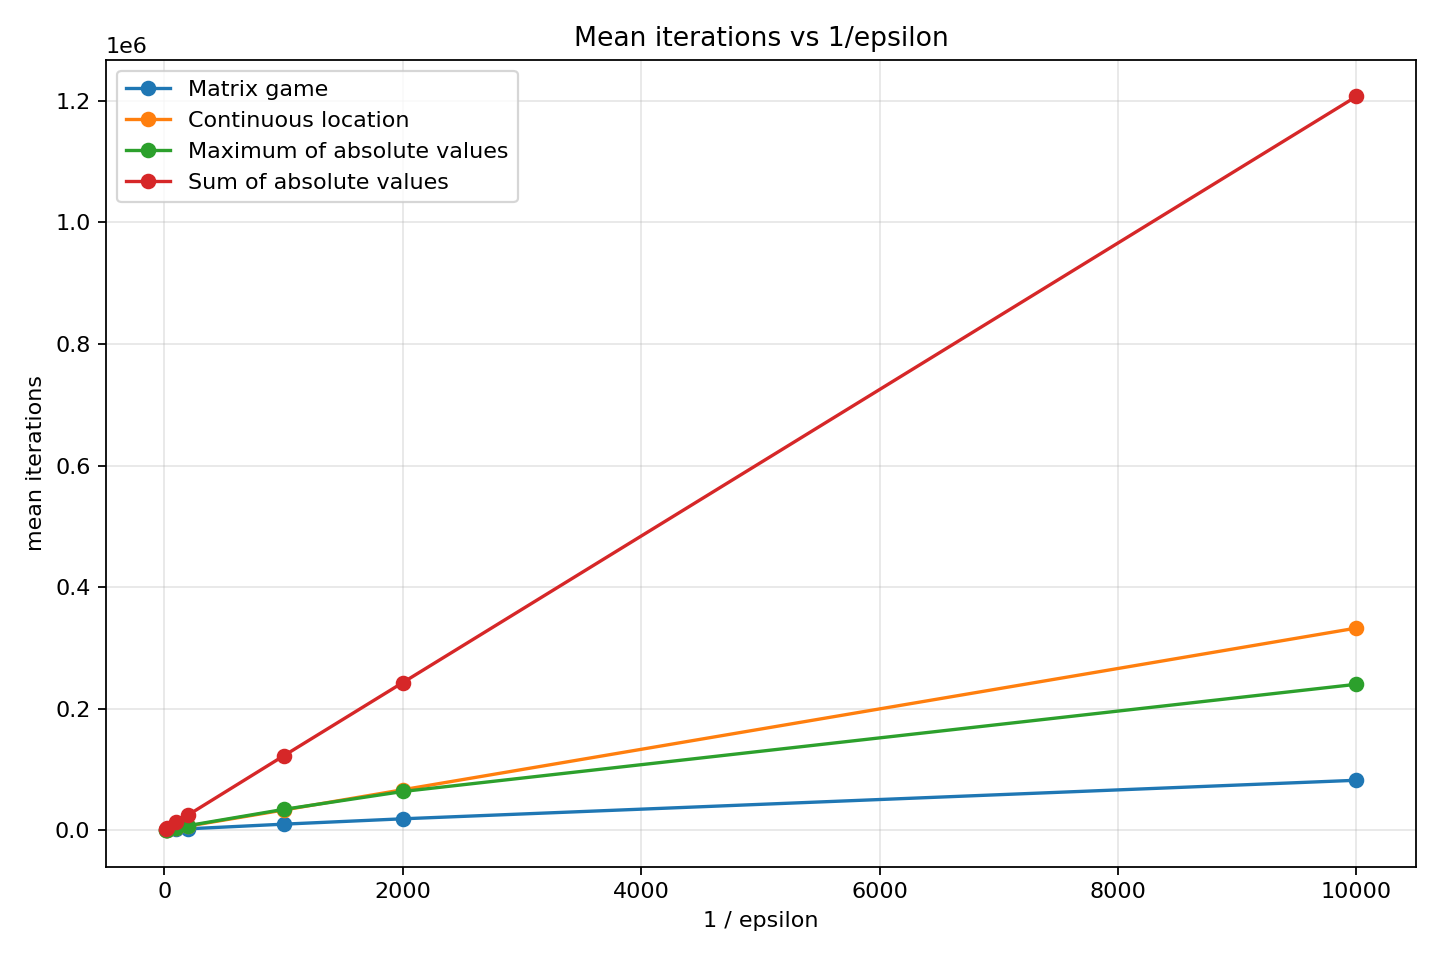
\includegraphics[width=0.85\textwidth]{results/plots/epsilon_scaling_iterations_vs_inverse_epsilon.png}
    \caption{Mean number of iterations versus \(1/\varepsilon\).}
    \label{fig:epsilon-scaling-linear}
\end{figure}

This plot gives a direct visual check of the theoretical prediction. If
\[
    N(\varepsilon)\approx C\frac{1}{\varepsilon},
\]
then the curves should be approximately linear in \(1/\varepsilon\). This is
what is observed for all four problem classes. The main difference between the
curves is the constant factor: the sum of absolute values problem requires the
most iterations, while the matrix game is the cheapest in this fixed-size test.
The overall shape is consistent with the expected complexity
\[
    N=O(1/\varepsilon).
\]


\subsubsection{Log-log plot and fitted exponent}

To examine the empirical rate more precisely, the iteration counts were also
analyzed on a log-log scale. If the number of iterations satisfies a relation of
the form

\[
    N(\varepsilon)\approx C\varepsilon^{-p},
\]

then taking logarithms gives

\[
    \log N
    =
    \log C+p\log(1/\varepsilon).
\]

Thus, the exponent \(p\) can be estimated as the slope of a linear regression
between \(\log N\) and \(\log(1/\varepsilon)\). The theoretical complexity
\(N=O(1/\varepsilon)\) corresponds to

\[
    p=1.
\]

The log-log plot is shown in Figure~\ref{fig:epsilon-scaling-loglog}. The
approximately linear shape of the curves confirms that a power-law model is a
reasonable description of the observed dependence on \(\varepsilon\).

\begin{figure}[H]
    \centering
    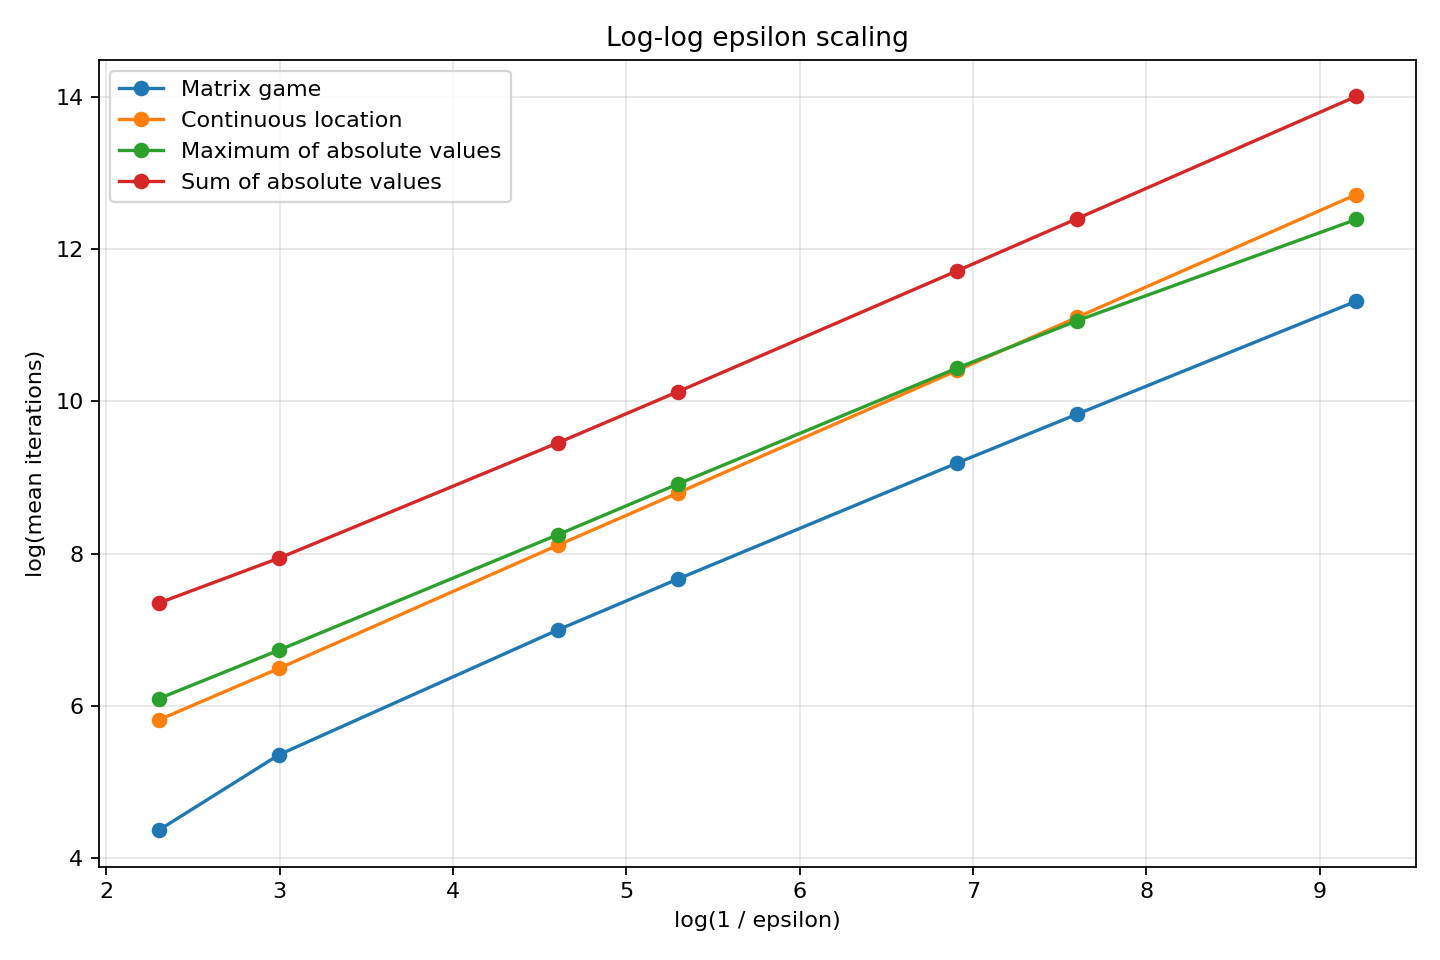
\includegraphics[width=0.85\textwidth]{results/plots/epsilon_scaling_loglog.png}
    \caption{Log-log plot for the epsilon-scaling experiment.}
    \label{fig:epsilon-scaling-loglog}
\end{figure}

The fitted exponents are shown in Table~\ref{tab:epsilon-scaling-regression}.
The table reports the estimated exponent \(\hat p\) and its standard error.

\begin{table}[H]
    \centering
    \begin{tabular}{lrrrr}
\toprule
Problem & $\hat p$ & SE \\
\midrule
Matrix game & 0.9897 & 0.0096 \\
Continuous location & 0.9986 & 0.0054 \\
Maximum of absolute values & 0.9208 & 0.0042 \\
Sum of absolute values & 0.9649 & 0.0096 \\
\bottomrule
\end{tabular}
    \caption{Fitted exponents in the empirical model
    \(N(\varepsilon)\approx C\varepsilon^{-p}\).}
    \label{tab:epsilon-scaling-regression}
\end{table}

The fitted exponents for the matrix game and continuous location problem are
very close to \(1\), which is consistent with the theoretical
\(O(1/\varepsilon)\) complexity. For the maximum of absolute values problem and
the sum of absolute values problem, the fitted exponents are slightly below
\(1\). This means that, for these random instances, the observed iteration
counts grew slightly slower than the worst-case \(1/\varepsilon\) rate.

Overall, the log-log analysis supports the theoretical prediction. The observed
rates are close to \(1/\varepsilon\), and in some cases slightly better. This is
consistent with the interpretation that the theoretical complexity bound is a
worst-case estimate and may be conservative on randomly generated instances.



\subsection{Experiment with changing the smoothing parameter \texorpdfstring{\(\mu\)}{mu}}

The previous experiments used Nesterov's smoothing method directly with
\[
    \mu_\varepsilon=\frac{\varepsilon}{2D_2}.
\]
This experiment compares that standard choice with the continuation strategy
from Section~\ref{sec:changing-mu}.

For the continuation runs, the smoothing parameter starts at
\[
    \mu_0=8\mu_\varepsilon
\]
and is then updated by
\[
    \mu_{t+1}=0.5\mu_t
\]
until \(\mu_\varepsilon\) is reached. The tested sequence is therefore
\[
    8\mu_\varepsilon,
    \quad
    4\mu_\varepsilon,
    \quad
    2\mu_\varepsilon,
    \quad
    \mu_\varepsilon.
\]
An intermediate stage is stopped when
\[
    f(\hat x)-\phi(\hat u)\le \mu_tD_2,
\]
and the final stage is stopped when
\[
    f(\hat x)-\phi(\hat u)\le \varepsilon.
\]
The experiment was performed for all four problem classes, using the same fixed
problem sizes as in the epsilon-scaling experiment:

\[
\begin{array}{l|c}
\text{Problem} & \text{Size}\\
\hline
\text{Matrix game} & m=300,\ n=1000\\
\text{Continuous location} & p=50,\ d=5,\ r=1\\
\text{Maximum of absolute values} & m=300,\ n=200,\ r=1\\
\text{Sum of absolute values} & m=300,\ n=200,\ r=1
\end{array}
\]

The tested accuracies were

\[
    \varepsilon\in\{10^{-2},10^{-3},10^{-4}\}.
\]

For each problem, each value of \(\varepsilon\), and each random seed, the same
random instance was solved twice: once with the standard smoothing method and
once with the continuation strategy. This makes the comparison fair, since both
runs solve the same instance.

\subsubsection{Iteration comparison}

Table~\ref{tab:mu-comparison-summary} reports the average number of iterations
for the standard smoothing method and for continuation.

\begin{table}[H]
    \centering
    \begin{tabular}{lclrr}
\toprule
Problem & $\varepsilon$ & $\mu$ mode & Mean iter. & Std iter. \\
\midrule
Continuous location & $10^{-4}$ & Continuation & 379\,813 & 37\,174 \\
Continuous location & $10^{-4}$ & Fixed $\mu$ & 306\,630 & 29\,498 \\
Continuous location & $10^{-3}$ & Continuation & 37\,330 & 10\,378 \\
Continuous location & $10^{-3}$ & Fixed $\mu$ & 30\,237 & 8\,283 \\
Continuous location & $10^{-2}$ & Continuation & 2\,923 & 1\,247 \\
Continuous location & $10^{-2}$ & Fixed $\mu$ & 3\,240 & 483.64 \\
Matrix game & $10^{-4}$ & Continuation & 115\,059 & 2\,313 \\
Matrix game & $10^{-4}$ & Fixed $\mu$ & 88\,760 & 1\,864 \\
Matrix game & $10^{-3}$ & Continuation & 12\,853 & 416.61 \\
Matrix game & $10^{-3}$ & Fixed $\mu$ & 9\,997 & 326.88 \\
Matrix game & $10^{-2}$ & Continuation & 1\,466 & 29.78 \\
Matrix game & $10^{-2}$ & Fixed $\mu$ & 1\,126 & 30.57 \\
Maximum of absolute values & $10^{-4}$ & Continuation & 331\,092 & 26\,995 \\
Maximum of absolute values & $10^{-4}$ & Fixed $\mu$ & 260\,380 & 18\,927 \\
Maximum of absolute values & $10^{-3}$ & Continuation & 44\,448 & 536.44 \\
Maximum of absolute values & $10^{-3}$ & Fixed $\mu$ & 34\,493 & 385.07 \\
Maximum of absolute values & $10^{-2}$ & Continuation & 5\,059 & 68.72 \\
Maximum of absolute values & $10^{-2}$ & Fixed $\mu$ & 3\,790 & 81.63 \\
Sum of absolute values & $10^{-4}$ & Continuation & 1\,679\,708 & 193\,437 \\
Sum of absolute values & $10^{-4}$ & Fixed $\mu$ & 1\,297\,689 & 147\,250 \\
Sum of absolute values & $10^{-3}$ & Continuation & 150\,866 & 7\,829 \\
Sum of absolute values & $10^{-3}$ & Fixed $\mu$ & 115\,690 & 6\,887 \\
Sum of absolute values & $10^{-2}$ & Continuation & 18\,853 & 2\,015 \\
Sum of absolute values & $10^{-2}$ & Fixed $\mu$ & 14\,448 & 1\,536 \\
\bottomrule
\end{tabular}
    \caption{Comparison of the standard smoothing method and continuation.}
    \label{tab:mu-comparison-summary}
\end{table}

The results show that continuation did not reduce the iteration count in most
cases. For the matrix game, the maximum of absolute values problem, and the sum
of absolute values problem, continuation required more iterations than the
standard method for all tested accuracies. The same pattern appears for the
continuous location problem at \(\varepsilon=10^{-3}\) and
\(\varepsilon=10^{-4}\). The only average improvement occurred for the
continuous location problem at \(\varepsilon=10^{-2}\).

For the tested instances and continuation parameters, the benefit of starting
with a smoother problem did not compensate for the extra work required by the
additional stages.

\subsubsection{Iteration speedup}

To make the comparison clearer, Table~\ref{tab:mu-comparison-speedup} reports
the iteration speedup

\[
    \text{speedup}
    =
    \frac{
        \text{iterations for the standard method}
    }{
        \text{iterations for continuation}
    }.
\]

Thus, values greater than \(1\) mean that continuation used fewer iterations,
while values below \(1\) mean that the standard method was better.

\begin{table}[H]
    \centering
    \begin{tabular}{lcrrr}
\toprule
Problem & $\varepsilon$ & Mean iter. speedup & Min iter. speedup & Max iter. speedup \\
\midrule
Continuous location & $10^{-4}$ & 0.807 & 0.806 & 0.810 \\
Continuous location & $10^{-3}$ & 0.811 & 0.806 & 0.818 \\
Continuous location & $10^{-2}$ & 1.28 & 0.804 & 1.89 \\
Matrix game & $10^{-4}$ & 0.771 & 0.768 & 0.774 \\
Matrix game & $10^{-3}$ & 0.778 & 0.772 & 0.782 \\
Matrix game & $10^{-2}$ & 0.768 & 0.759 & 0.778 \\
Maximum of absolute values & $10^{-4}$ & 0.787 & 0.775 & 0.792 \\
Maximum of absolute values & $10^{-3}$ & 0.776 & 0.770 & 0.781 \\
Maximum of absolute values & $10^{-2}$ & 0.749 & 0.740 & 0.759 \\
Sum of absolute values & $10^{-4}$ & 0.773 & 0.764 & 0.779 \\
Sum of absolute values & $10^{-3}$ & 0.767 & 0.756 & 0.778 \\
Sum of absolute values & $10^{-2}$ & 0.766 & 0.758 & 0.773 \\
\bottomrule
\end{tabular}
    \caption{Iteration speedup of continuation relative to the standard smoothing method.}
    \label{tab:mu-comparison-speedup}
\end{table}

The speedup table confirms the previous observation. Most speedup values are
below \(1\), usually around \(0.75\)--\(0.81\). This means that continuation
typically required about \(20\%\)--\(30\%\) more iterations than the standard
method. The only average speedup above \(1\) occurs for the continuous
location problem with \(\varepsilon=10^{-2}\), where the mean speedup is
approximately \(1.28\). However, even in this case the minimum speedup is below
\(1\), so the improvement was not consistent across all seeds.

Overall, this experiment suggests that the standard smoothing method is more
efficient for the tested settings.

\subsubsection{Gap history}

In addition to final iteration counts, the primal-dual gap was tracked during
optimization for representative runs with

\[
    \varepsilon=10^{-4},
    \qquad
    \text{seed}=0.
\]

This gives more detailed information about the behavior of both methods. The
following plots show the primal-dual gap as a function of the iteration number.
The \(y\)-axis is logarithmic, and the horizontal dotted line marks the target
accuracy \(\varepsilon=10^{-4}\). For the continuation method, vertical dotted
lines indicate changes of the smoothing parameter \(\mu\).

\begin{figure}[H]
    \centering
    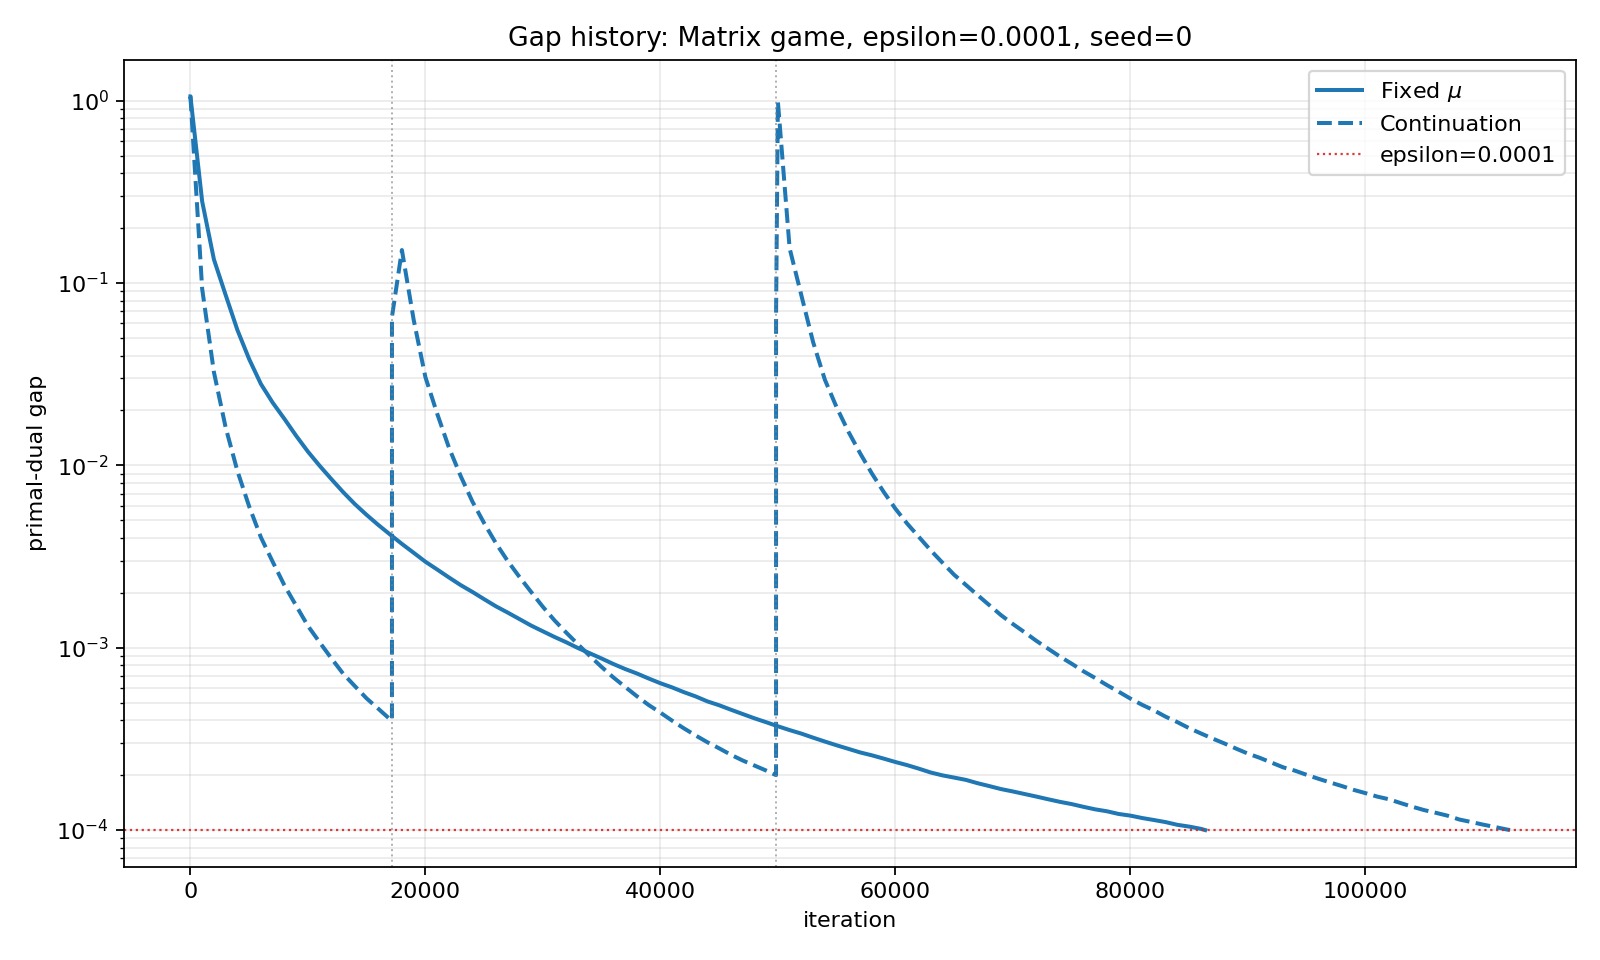
\includegraphics[width=0.9\textwidth]{results/plots/mu_gap_history_matrix_game_eps_1e-04.png}
    \caption{Gap history for the matrix game with $\varepsilon=10^{-4}$.}
    \label{fig:mu-gap-history-matrix-game}
\end{figure}

\begin{figure}[H]
    \centering
    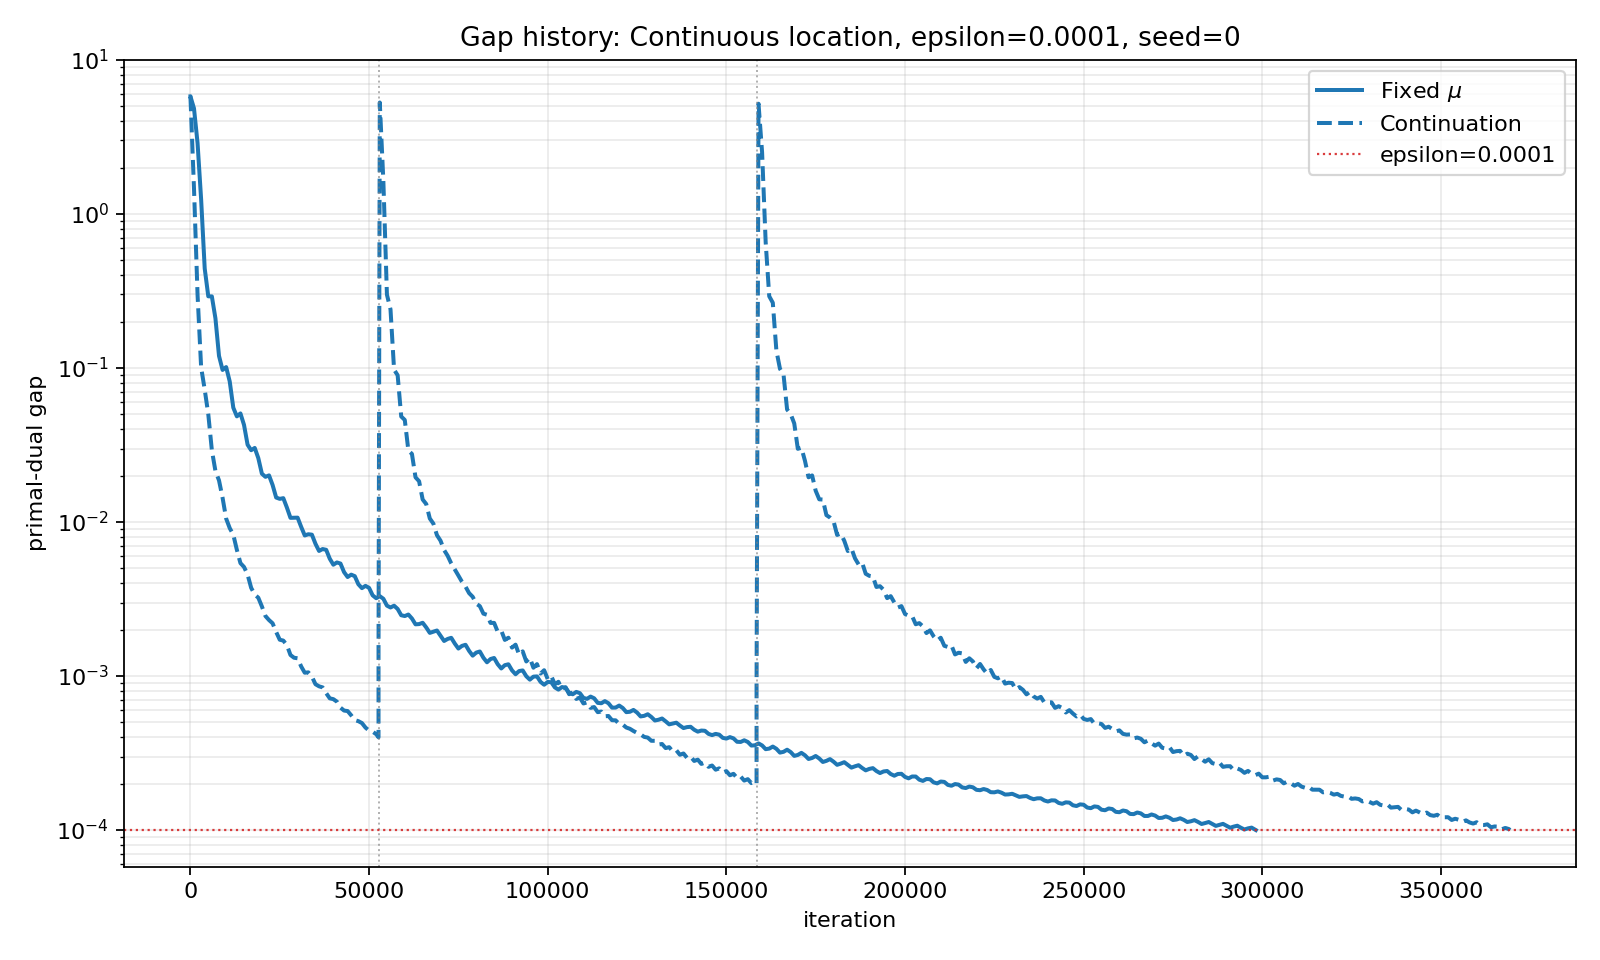
\includegraphics[width=0.9\textwidth]{results/plots/mu_gap_history_continuous_location_eps_1e-04.png}
    \caption{Gap history for the continuous location problem with
    $\varepsilon=10^{-4}$.}
    \label{fig:mu-gap-history-continuous-location}
\end{figure}

\begin{figure}[H]
    \centering
    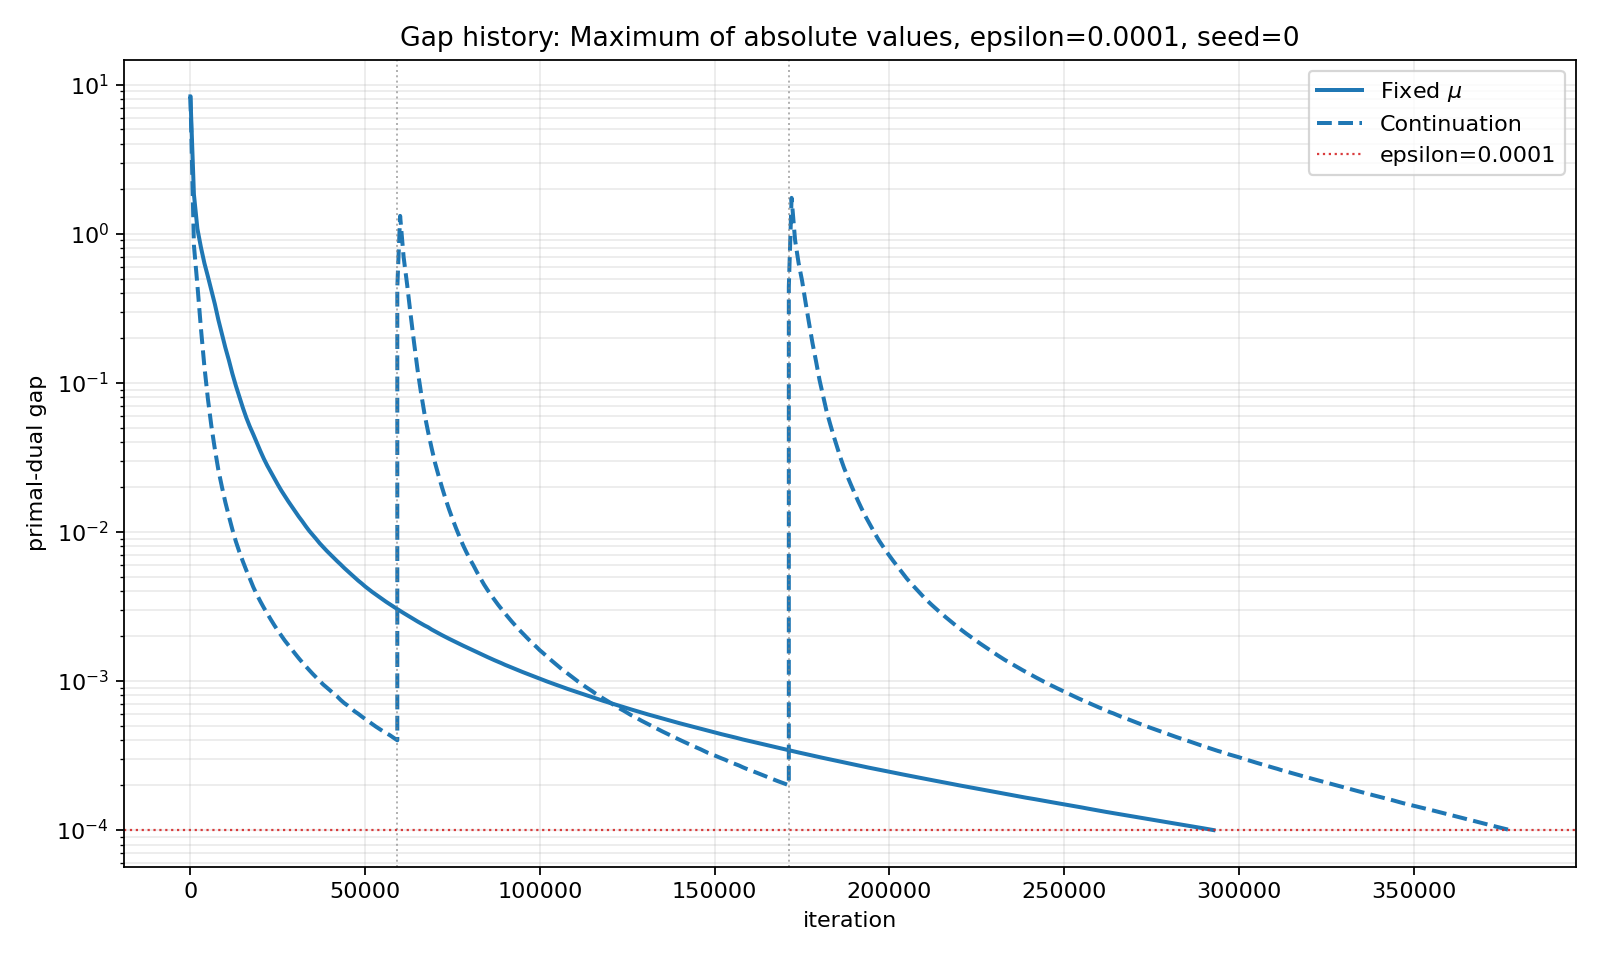
\includegraphics[width=0.9\textwidth]{results/plots/mu_gap_history_piecewise_linear_max_abs_eps_1e-04.png}
    \caption{Gap history for the maximum of absolute values problem with
    $\varepsilon=10^{-4}$.}
    \label{fig:mu-gap-history-piecewise}
\end{figure}

\begin{figure}[H]
    \centering
    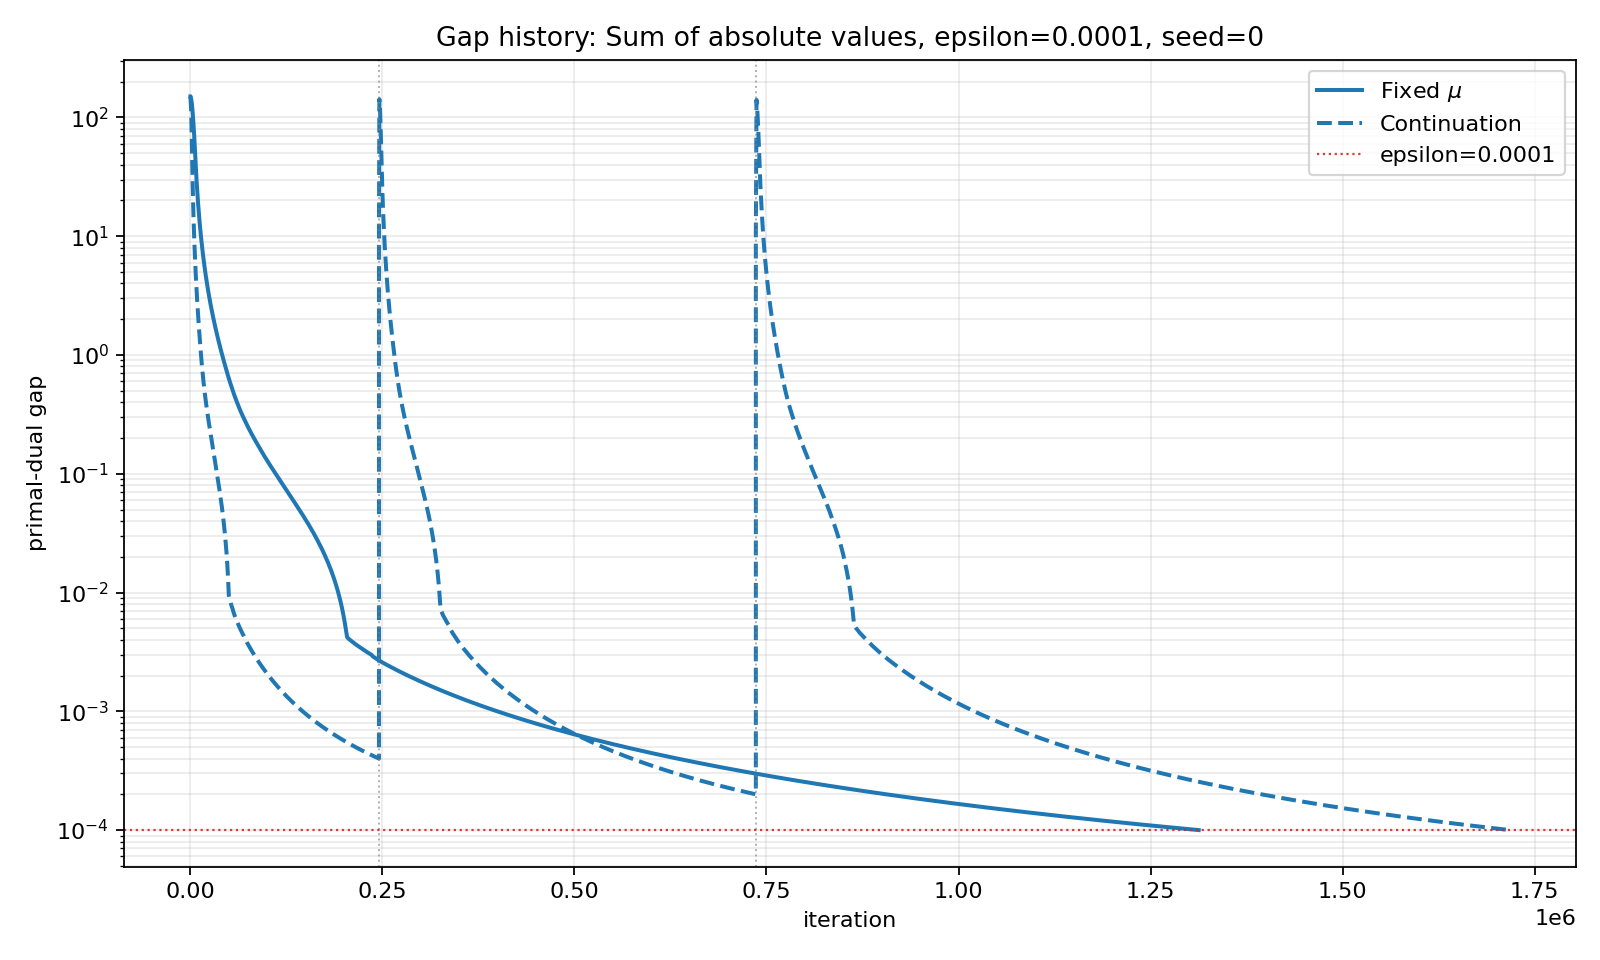
\includegraphics[width=0.9\textwidth]{results/plots/mu_gap_history_sum_absolute_eps_1e-04.png}
    \caption{Gap history for the sum of absolute values problem with
    $\varepsilon=10^{-4}$.}
    \label{fig:mu-gap-history-sum-absolute}
\end{figure}

The plots show that continuation reduces the gap quickly inside each stage, but
after each decrease of \(\mu\), the gap increases again. This is expected:
changing \(\mu\) changes the smoothed objective and makes the approximation
closer to the original non-smooth function. Therefore, the current point may no
longer have as small a gap for the new, less smoothed problem.

For the tested instances, the standard smoothing method reaches the target line
earlier than continuation. This is especially clear for the matrix game,
maximum of absolute values problem, and sum of absolute values problem. In
the continuous location problem, the difference is smaller, but the standard method
still reaches the final tolerance earlier for the displayed
\(\varepsilon=10^{-4}\) run.


\section{Discussion and conclusion}

The experiments support the main theoretical message of Nesterov's smoothing
method. For all tested reproduction-style instances, the algorithm reached the
required primal-dual gap. This means that the stopping criterion provided a
certificate of solution quality. At the same time, the observed iteration counts
were substantially smaller than the worst-case predictions. This is natural,
since the theoretical bound is designed for the worst case, while the numerical
tests use randomly generated instances.

The fixed-size epsilon-scaling experiment gives the clearest evidence for the
predicted dependence on the accuracy parameter. For the matrix game and the
continuous location problem, the fitted exponents were very close to \(1\), in
agreement with the theoretical \(O(1/\varepsilon)\) complexity. For the maximum
of absolute values and the sum of absolute values problems, the fitted
exponents were slightly below \(1\). This does not contradict the theorem; it
only means that the observed growth was somewhat better than the worst-case rate
on these instances.

The comparison between problem classes shows that the hidden constants are
important in practice. The sum of absolute values problem required many more
iterations than the other examples, even though its empirical dependence on
\(\varepsilon\) remained close to linear. This reflects the structure of the
objective. The maximum of absolute values problem depends on the largest
residual, whereas the sum of absolute values problem aggregates all residuals.
This can lead to a larger effective Lipschitz constant after smoothing and
therefore to a larger number of iterations.

The continuation experiment shows that changing the smoothing parameter is not
automatically beneficial. Although larger values of \(\mu\) make the early
smoothed problems easier, the method must solve several stages. In addition,
when \(\mu\) is reduced, the smoothed approximation changes and the
primal-dual gap can increase. With the tested schedule
\(\mu_0=8\mu_\varepsilon\) and decay factor \(0.5\), the standard smoothing
method was usually more efficient. Continuation should therefore be treated as
a heuristic whose performance depends on the chosen schedule and intermediate
stopping rules.

Overall, the implementation confirms that Nesterov's smoothing framework is a
useful approach for structured non-smooth convex optimization. It gives a
systematic way to replace a non-smooth max-term by a smooth approximation, apply
an accelerated first-order method, and stop with a certified primal-dual gap.
The experiments are consistent with the theoretical \(O(1/\varepsilon)\) rate
and show that the method is effective for several different problem structures.
They also show that practical performance depends on the objective structure and
on the choice of smoothing strategy.

\bibliographystyle{plain}
\bibliography{references}

\end{document}
